\documentclass[a4paper, twoside, 11pt]{report}

\usepackage[utf8]{inputenc}
\usepackage[T1]{fontenc}
\usepackage[english]{babel}
\usepackage[top= 120pt, left=80pt, right=80pt]{geometry} %marges
\usepackage{setspace} %interlignage
\usepackage{url}
\usepackage{graphicx}
\usepackage{lmodern} 
\usepackage{array}
\usepackage{csquotes}
\usepackage[numbers,square]{natbib}
\usepackage{soul}
\usepackage{hyperref}
\usepackage{amsthm}
\usepackage{color}
\usepackage[usenames,dvipsnames,svgnames,table]{xcolor}
\usepackage{adjustbox}
\usepackage{amssymb}
\usepackage{amsmath}
\usepackage{dsfont}
%%\usepackage{braket}
\usepackage{physics}
\usepackage{amsfonts}
\usepackage[numbers,square]{natbib}
\usepackage{multirow}
\usepackage{listings}
\usepackage{wasysym}
\usepackage{algpseudocode}
\usepackage[ruled]{algorithm2e}
\usepackage{caption}


%%%%%% COULEURS CODE C++
\lstdefinestyle{customc}{
  belowcaptionskip=1\baselineskip,
  breaklines=true,
  frame=L,
  xleftmargin=\parindent,
  language=C,
  showstringspaces=false,
  basicstyle=\footnotesize\ttfamily,
  keywordstyle=\bfseries\color{red},
  commentstyle=\itshape\color{gray},
  identifierstyle=\color{NavyBlue},
  stringstyle=\color{black},
}

\lstdefinestyle{customasm}{
  belowcaptionskip=1\baselineskip,
  frame=L,
  xleftmargin=\parindent,
  language=[x86masm]Assembler,
  basicstyle=\footnotesize\ttfamily,
  commentstyle=\itshape\color{purple!40!black},
}

\lstset{escapechar=@,style=customc}

%%%%%% STYLES DE THÉORÈMES

\newtheoremstyle{theorem}%	Name
  {}%	Space above
  {}%	Space below
  {}%	Body font
  {}%	Indent amount
  {\bfseries}%	Theorem head font
  {.}%	Punctuation after theorem head
  { }%	Space after theorem head, ' ', or \newline
  {}%	Theorem head spec (can be left empty, meaning `normal')

\newtheoremstyle{exemple}%	Name
  {}%	Space above
  {}%	Space below
  {\color{Gray}\itshape}%	Body font
  {}%	Indent amount
  {\color{Gray}\itshape}%	Theorem head font
  {.}%	Punctuation after theorem head
  { }%	Space after theorem head, ' ', or \newline
  {}%	Theorem head spec (can be left empty, meaning `normal')

\newtheoremstyle{remark}%	Name
  {}%	Space above
  {}%	Space below
  {\itshape}%	Body font
  {}%	Indent amount
  {\bfseries}%	Theorem head font
  {.}%	Punctuation after theorem head
  { }%	Space after theorem head, ' ', or \newline
  {}%	Theorem head spec (can be left empty, meaning `normal')
  
%%%%%% DÉCLARATION DES THÉORÈMES

\theoremstyle{theorem}
\newtheorem{theorem}{Theorem}[section]
\newtheorem{lemme}{Lemma}[section]
\newtheorem{proposition}{Proposition}[section]
\newtheorem{definition}{Definition}[section]

\theoremstyle{remark}
\newtheorem{remark}{Remark}[chapter]

\theoremstyle{exemple}
\newtheorem*{exemple}{Example}


%%%%%% COMMANDES QUI SIMPLIFIENT LA VIE

\newcommand{\legende}[1]{
\begin{center}
	\begin{minipage}{12cm}
		\begin{center}
			\textit{\textcolor{WildStrawberry!30}{#1}}
		\end{center}
	\end{minipage}
\end{center}}

\newcommand{\sherlock}[2]{
	\begin{equation}
		\textcolor{WildStrawberry}{#1}
	\end{equation}
	\legende{#2}
}
	
\newcommand{\sherlocked}[1]{
	\begin{equation}
		\textcolor{WildStrawberry}{#1}
	\end{equation}
}

	
\newcommand{\defSherlock}[3]{
	\begin{definition}[\textbf{#1}]
		\sherlock{#2}{#3}
	\end{definition}
}

\newcommand{\defSherlocked}[2]{
	\begin{definition}[\textbf{#1}]
		\sherlocked{#2}
	\end{definition}
}	

\newcommand{\propSherlock}[3]{
	\begin{proposition}[\textbf{#1}]
		\sherlock{#2}{#3}
	\end{proposition}
}

\newcommand{\propSherlocked}[2]{
	\begin{proposition}[\textbf{#1}]
		\sherlocked{#2}
	\end{proposition}
}

\newcommand{\textSherlocked}[1]{
	\begin{center}
		\textcolor{WildStrawberry}{#1}
	\end{center}
}

\newcommand{\mimi}{\mathrm{Je\ t'aime}}

\newcommand{\N}{\mathbb{N}}
\newcommand{\Z}{\mathbb{Z}}
\newcommand{\R}{\mathbb{R}}
\newcommand{\C}{\mathbb{C}}

\newcolumntype{M}[1]{>{\centering\arraybackslash}m{#1}} %Pour personnaliser la largeur des colonnes dans des tabular tout en restant centré



%%%%%%%%%%%%%%%%%%%%%%%%%%%%%%%%%%%%%%%%%%%%%%%%%%%%%%%
%%%%%%%%%%%%%%%%%%%%%%%%%%%%%%%%%%%%%%%%%%%%%%%%%%%%%%%
%%%%%%%%%%%%%%%%%%%%%%%%%%%%%%%%%%%%%%%%%%%%%%%%%%%%%%%

\title{FYS3150\\Project 4 - }
\author{Ethel Villeneuve}
\date{October 2017 \\University of Oslo \\ \url{https://github.com/choukimono/Project_4.git}}



\begin{document}
\selectlanguage{english}
\maketitle
	
	
\begin{abstract}
    
    \paragraph{}In this project, we want to implement the Ising model, in the case of a two-dimensional squared lattice, with periodic boundary conditions, by using the object-oriented programming. In this lattice, we have $L\times L$ particles characterized by their spin (up or down). The starting point of the program will be a random lattice or a lattice with all the spins-up. The Metropolis algorithm will be run in a lattice $20\times20$ and then bigger. We will study the properties of the system : the mean energy $E$, the mean magnetization $|M|$, the specific heat and the susceptibility $\chi$ as function of the temperature. The purpose is then to study the phase transitions. We will again study these properties near the critical temperature (Curie point).
    
    \paragraph{}Quelques résultats...
    
\end{abstract}


\tableofcontents


\chapter*{Introduction}
\addcontentsline{toc}{chapter}{Introduction}

    \paragraph{}
    

\chapter{Theory}
    
    \section{The Ising model}
    
        \subsection{The general model}
        
            \paragraph{}The Ising model is a mathematical model used in statistical mechanics. It consists of discrete variables, which represent the magnetic moment of the spin, which can take only two values (here $+1$ or $-1$). The spins will only interact with their direct neighbors. With this model, we can study the phase transitions at finite temperature for magnetic systems. We can expressed the energy as 
                
                \begin{equation*}
                    E = -J \sum\limits_{\langle  kl\rangle}^{N}s_ks_l - B \sum\limits_{k}^{N}s_k
                    \tag{1}
                \end{equation*}
            %Mets pas de saut de ligne ici patate, ça évitera l'alinéa moche.
            with $J$ a constant expressing the strength of the interaction between the neighboring spins, $\langle kl \rangle$ indicating the fact that we only sum the nearest neighbors, $N$ the number of spins, $s_{k,l} = \pm 1$ and $B$ an external magnetic field interacting with the magnetic moment set up by the spins. This is the general expression of the Ising model. For our use, we will only focus on the case where $B=0$. \\
            Then, we will be able to calculate expectation values of the mean energy $\langle E \rangle$ and magnetization $\langle M \rangle$ at a given temperature. To do this, we will use a Boltzmann distribution
            %
                \begin{equation*}
                    P_i(\beta) = \frac{e^{-\beta E_i}}{Z}
                    \tag{2}
                \end{equation*}
             %blblbl
            where $P_i$ is the probability of finding the system in the state $i$, $\beta = \frac{1}{kT}$, $T$ being the temperature and $k$ the Boltzmann constant, $E_i$ is the energy of a state $i$ and $Z$ is the partition function defined by $\displaystyle Z = \sum\limits_{i=1}^{M}e^{-\beta E_i}$ with $M$ the number of configurations. $E_i$, which is the energy in the state $i$, is given by, for $k$, $l$ the spins of the state $i$ : 
            %
                \begin{equation*}
                    E_i = -J \sum\limits_{\langle kl \rangle}^{N}s_ks_l 
                    \tag{3}
                \end{equation*} 
            A simple particular case of the Ising model, the two-dimensional square lattice model, allows us to have an analytical solution, which will be compared to the numerical results.
        
        \subsection{Two-dimensional square lattice model}
        
            \paragraph{}This particular case is one of the simplest models to show a phase transition. It is defined by the following conditions : a null external magnetic field $B=0$, this is a two-dimensional lattice with $N = L\times L$ sites with $L$ the number of spins in each dimension, with periodic boundary conditions. \\
            Let's take the case with $N=2\times2$ spins. We have $2^4 = 16$ different possible states with those conditions. We reuse the equation (3) to find the energy of each configuration $i$ with the spins-up $\uparrow$ taking the value $+1$ and the spins-down $\downarrow$ taking the value $-1$. Let's take for example the case where three spins are pointing up (and so one is pointing down) numbered from 1 to 4 :
                $\begin{matrix}
                    \downarrow ^{(1)} & \uparrow ^{(2)}\\
                    \uparrow ^{(3)} & \uparrow ^{(4)}
                \end{matrix}$.
            %    
                \begin{align*}
                    E &= -J \sum\limits_{\langle kl \rangle}^{4}s_ks_l \\
                      &= -J (s_1s_2 + s_2s_1 + s_1s_3 + s_3s_1 + s_2s_4 + s_4s_2 + s_3s_4 + s_4s_3) \\
                      &= -J \left[(-1) + (-1) + (-1) + (-1) + 1 + 1 + 1 + 1\right] \\
                      &= -J \times 0 \\
                    \underline{E\ }&\underline{=}\underline{\ 0} 
                \end{align*}
            %    
            The magnetization formula is the simple sum of all spin of the state $\displaystyle M = \sum\limits_{k}^{N} s_k$ with $k$ each spin of the configuration. So in our example, we have 
            %    
                \begin{align*}
                    M &= s_1 + s_2 + s_3 + s_4 \\
                      &= (-1) + 1 + 1 + 1 \\
                    \underline{M\ }&\underline{=}\underline{\ 2}
                \end{align*}
            %
            \paragraph{}The following table sums up the possible states of a two-dimensional square lattice model.
            %
                \begin{center}
                    \begin{tabular}{|*{8}{c|}}
                            \hline
                        Number of spins-up & \multicolumn{4}{c|}{Possible configurations} & Degeneracy & Energy & Magnetization \\
                            \hline
                            \hline
                        $4$ & \multicolumn{4}{c|}{$\begin{matrix}
                                   \uparrow & \uparrow \\
                                   \uparrow & \uparrow
                                \end{matrix}$} & $1$ & $-8J$ & $4$ \\
                            \hline
                        $3$ & $\begin{matrix}
                            \downarrow & \uparrow \\
                            \uparrow & \uparrow
                        \end{matrix}$ & $\begin{matrix}
                                            \uparrow & \downarrow \\
                                            \uparrow & \uparrow
                                         \end{matrix}$ & $\begin{matrix}
                                                               \uparrow & \uparrow \\
                                                               \downarrow & \uparrow
                                                           \end{matrix}$ & $\begin{matrix}
                                                                                \uparrow & \uparrow \\
                                                                                \uparrow & \downarrow
                                                                            \end{matrix}$ & $4$ & $0$ & $2$ \\
                            \hline
                        $2$ & $\begin{matrix}
                                   \uparrow & \uparrow \\
                                   \downarrow & \downarrow
                               \end{matrix}$ & $\begin{matrix}
                                                     \downarrow & \downarrow \\
                                                     \uparrow & \uparrow
                                                \end{matrix}$ & $\begin{matrix}
                                                                    \uparrow & \downarrow \\
                                                                    \uparrow & \downarrow
                                                                 \end{matrix}$ & $\begin{matrix}
                                                                     \downarrow & \uparrow \\
                                                                     \downarrow & \uparrow
                                                                \end{matrix}$ & $4$ & $0$ & $0$ \\
                            \hline
                        $2$ & \multicolumn{2}{c|}{$\begin{matrix}
                                    \uparrow & \downarrow \\
                                    \downarrow & \uparrow
                                \end{matrix}$} & \multicolumn{2}{c|}{$\begin{matrix}
                                                     \downarrow & \uparrow \\
                                                     \uparrow & \downarrow
                                                  \end{matrix}$} & $2$ & $8J$ & $0$ \\
                            \hline
                        $1$ & $\begin{matrix}
                            \downarrow & \downarrow \\
                            \downarrow & \uparrow
                        \end{matrix}$ & $\begin{matrix}
                                            \downarrow & \downarrow \\
                                            \uparrow & \downarrow
                                         \end{matrix}$ & $\begin{matrix}
                                                               \downarrow & \uparrow \\
                                                               \downarrow & \downarrow
                                                           \end{matrix}$ & $\begin{matrix}
                                                                                \uparrow & \downarrow \\
                                                                                \downarrow & \downarrow
                                                                            \end{matrix}$ & $4$ & $0$ & $-2$ \\
                            \hline
                        $0$ & \multicolumn{4}{c|}{$\begin{matrix}
                                                       \downarrow & \downarrow \\
                                                       \downarrow & \downarrow
                                                     \end{matrix}$} & $1$ & $-8J$ & $-4$ \\
                            \hline            
                    \end{tabular}
                \captionof{table}{Energy and magnetization for a $N = 2\times 2$ spins Ising model with periodic boundary conditions.}
                \end{center}
            
            The 16 configurations known, we can calculate the partition function in its analytic form. 
            %
                \begin{align*}
                    Z &= \sum\limits_{i=1}^{16}e^{-\beta E_i} \\
                    Z &= (1 \times e^{-\beta \times (-8J)}) + (4 \times e^{-\beta \times 0}) + (4 \times e^{-\beta \times 0}) + (2 \times e^{-\beta \times 8J}) + (4 \times e^{-\beta \times 0}) + (1 \times e^{-\beta \times (-8J)})        
                \end{align*}
            %    
                \begin{align*}
                    &\boxed{Z = 2(e^{8J\beta} + e^{-8J\beta} + 6)} \tag{4}\\
                    &Z = 4[\cosh(8J\beta) + 3] \tag{4'}
                \end{align*}
                
            Let's now compute the expectation value of the energy, defined by
            
                \begin{equation*}
                    \langle E \rangle = \sum\limits_{i=1}^{M}E_iP_i(\beta)
                \end{equation*}            
            
            From (2), we can write :
            %
                \begin{align*}
                    \langle E \rangle &= \frac{1}{Z}\sum\limits_{i=1}^{M} E_i e^{-\beta E_i} \\
                    &= \frac{1}{Z} \left(2 \times (-8J) e^{8J\beta} + 2 \times 8J e^{-8J\beta}\right)
                \end{align*}             
            
                \begin{equation*}
                    \boxed{\langle E \rangle = -\frac{J}{Z}\left(16e^{8J\beta} - 16 e^{-8J\beta}\ \right)} 
                    \tag{5}
                \end{equation*}
                
                \begin{equation*}
                    \langle E \rangle = -8J \frac{e^{8J\beta} - e^{-8J\beta}}{e^{8J\beta} + e^{-8J\beta} + 6}
                \end{equation*}
            %            
                \begin{equation*}
                    \langle E \rangle =\ -8J \frac{\sinh (8J\beta)}{\cosh (8J\beta) + 3}  \tag{5'}
                \end{equation*}
            
            Similarly, we compute the mean value of the magnetic moment (or mean magnetization) in its absolute value $\langle |M| \rangle$ :
            
                \begin{equation*}
                    \langle |M| \rangle = \sum\limits_{i=1}^{M}|M_i|P_i(\beta) = \frac{1}{Z}\sum\limits_{i=1}^{M}|M_i| e^{-\beta E_i}
                \end{equation*}
                
                \begin{equation*}
                    \langle |M| \rangle = \frac{1}{Z} \left(4 e^{8J\beta} + 4 \times 2 e^{0} + 4 \times 2 e^{0} + 4 e^{8J\beta}\right) 
                \end{equation*}
                
                \begin{equation*}
                    \boxed{\langle |M| \rangle =\ \frac{8e^{8J\beta}+16}{Z}} 
                    \tag{6} 
                \end{equation*}
                
                \begin{equation*}
                    \langle |M| \rangle = \frac{4e^{8J\beta}+8}{e^{8J\beta}+e^{-8J\beta}+6}
                \end{equation*}
            %
            which match with the fact that we have taken the external magnetic field $B=0$.
            
            We can use the expression of the expectation value of the energy to find the specific heat $C_V$ which is defined by
            %
                \begin{equation*}
                    C_V = \frac{\langle E^2 \rangle - \langle E \rangle ^2}{kT^2}
                \end{equation*}
                
            The specific heat capacity represents the amount of energy requiered to raise the temperature of a unit of mass by a unit of temperature. 
                
            We need to compute $\langle E^2 \rangle$ :
                
                \begin{align*}
                    \langle E^2 \rangle &= \sum\limits_{i=1}^{M}E_i^2P_i(\beta) =\frac{1}{Z}\sum\limits_{i=1}^{M}E_i^2 e^{-\beta E_i} \\
                    &= \frac{1}{Z}\left(2 \times (-8J)^2 e^{8J\beta} + 2 \times (8J)^2 e^{-8J\beta} \right)
                \end{align*}
                
                \begin{equation*}
                    \boxed{\langle E^2 \rangle = \frac{J^2}{Z}\left(128e^{8J\beta} + 128e^{-8J\beta}\right)} 
                    \tag{7}
                \end{equation*}
                
                \begin{equation*}
                    \langle E^2 \rangle = 64J^2 \frac{e^{8J\beta} + e^{-8J\beta}}{e^{8J\beta} + e^{-8J\beta} + 6}
                \end{equation*}
                
                \begin{equation*}
                    \langle E^2 \rangle = 64J^2 \frac{\cosh(8J\beta)}{\cosh(8J\beta) +3} \tag{7'}
                \end{equation*}
            
            Then, with (5), we have
            
                \begin{equation*}
                    C_V = \frac{J^2}{ZkT^2}\left[\left[128\left(e^{8J\beta} + e^{-8J\beta}\right)\right] - \frac{1}{Z}\left[16\left(e^{8J\beta}-e^{-8J\beta}\right)\right]^2\right]   
                \end{equation*}
                
                \begin{equation*}
                    \boxed{C_V = \frac{256J^2}{ZkT^2}\left[\cosh(8J\beta) - \frac{4}{Z}\sinh^2(8J\beta)\right]}
                    \tag{8}
                \end{equation*}
                
            Similarly, to have the susceptibility $\chi$, which is its capacity to be attracted or not into a magnetic field, defined by
            
                \begin{equation*}
                    \chi = \frac{\langle |M|^2 \rangle - \langle |M| \rangle ^2}{kT},
                \end{equation*}
            %
            we start by computing $\langle |M|^2 \rangle$ :
            
                \begin{align*}
                    \langle |M|^2 \rangle &= \sum\limits_{i=1}^{M} |M_i|^2P_i(\beta) = \frac{1}{Z}\sum\limits_{i=1}^{M}|M_i|^2 e^{-\beta E_i} \\
                    &= \frac{1}{Z}\left(4^2e^{8J\beta} + 4 \times 2^2 e^{0} + 4 \times 2^2 e^{0} + 4^2e^{8J\beta}\right) 
                \end{align*}
                
                \begin{align*}
                    &\boxed{\langle |M|^2 \rangle = \frac{1}{Z}\left( 32e^{8J\beta} + 32 \right)} \tag{9}\\
                    &\langle |M|^2 \rangle = 16 \frac{e^{8J\beta}+1}{e^{8J\beta} + e^{-8J\beta} + 6}
                \end{align*}
                
            Using (6), we can write
            
                \begin{align*}
                    &\boxed{\chi = \frac{1}{ZkT}\left[\left(32e^{8J\beta}+32\right)-\frac{1}{Z}\left(8e^{8J\beta}+16\right)^2\right]} \tag{10}\\
                    &\chi = \frac{16}{kT}\left[\frac{3e^{8J\beta}+e^{-8J\beta}+3}{(e^{8J\beta}+e^{-8J\beta}+6)^2}\right]
                \end{align*}            
            

    \section{Phase transition}
    
        \paragraph{}A phase transition is a transformation of a system due to a variation of an external parameter (such as the temperature). It exists a critical point where the transition takes place. 
    
        \subsection{The critical temperature}
        
            \paragraph{}To study the phase transitions, we consider a critical temperature. The Ising model with our conditions (in two dimensions and with an null-external magnetic field $B=0$) undergoes a phase transition of second-order, called like this because of the fact that there is a discontinuity in the second derivative of the free energy. That means that the new states grows continuously from the previous one and when $T \rightarrow T_C$, these two states are quantatively the same. 
            
            \paragraph{}Near this temperature, a power-law applies to many physical quantities : one quantity varies as the power of another. In the Ising model, we can express the mean magnetization as 
                
                \begin{equation*}
                    \langle M(T)\rangle \sim (T-T_C)^{\beta}
                \end{equation*}
            %
            with $\displaystyle \beta = \frac{1}{8}$ one of the Ising critical exponents (in two dimensions).\\
            We have similar expression for the heat capacity and the susceptibility : 
            
                \begin{equation*}
                    C_V(T) \sim |T_C - T | ^{-\alpha}
                \end{equation*}
                
                \begin{equation*}
                    \chi(T) \sim |T_C - T |^{-\gamma}
                \end{equation*}
            %
            with $\displaystyle \alpha = 0$ and $\displaystyle \gamma=\frac{7}{4}$ two other critical exponents.\\
            We also defined the correlation length which is a quantity which represents how two spins are correlated. When the temperature $T$ gets closer to $T_C$, the correlation length between two spins increases. This quantity is given by 
            
                \begin{equation*}
                    \xi (T) \sim |T_C - T |^{-\nu},
                \end{equation*}
            %
            defining the constant $\nu$.
            
        \subsection{Around the critical temperature}            
            
            \paragraph{}When the correlation length spans the whole system, we say that we have a second-order (or continuous) phase transition. $\xi$ is proportional to the size of the lattice $L$ at the critical point ($\xi \propto L$), as it is always finite. With the finite size scaling relations, we can relate the temperature for a finite lattice and the one for an infinite lattice :
            
                \begin{equation*}
                    T_C(L) - T_C (L=\infty) = aL^{-\frac{1}{\nu}}
                \end{equation*}
            %
            with $a$ a constant.\\
            With the last equation, we can write :
            
                \begin{equation*}
                    \langle M(T) \rangle \sim (T-T_C)^{\beta} \rightarrow L^{-\frac{\beta}{\nu}}
                \end{equation*}
                
                \begin{equation*}
                    C_V(T) \sim |T_C -T|^{-\alpha} \rightarrow L^{\frac{\alpha}{\nu}}
                \end{equation*}
                
                \begin{equation*}
                    \chi(T) \sim |T_C - T|^{-\gamma} \rightarrow L^{\frac{\gamma}{\nu}}
                \end{equation*}
            %
            for $T$ near $T_C$.
            
            \paragraph{}To find the critical temperature of our case, we will plot the values of the physical properties we study from the beginning (namely the expectation values for the energy $E$ and the magnetic moment $|M|$, the specific heat $C_V$ and the susceptibility $\xi$ as function of the temperature $T$. The discontinuity in the graph would tell us an approximation of the critical temperature. We have a theorical value of the critical temperature which is 
                
                \begin{equation*}
                    \frac{kT_C}{J} = \frac{2}{\textnormal{ln}(1+\sqrt{2})} \approx 2.269
                    \tag{11}
                \end{equation*}
            %
            according to the work of Lars Onsager exposed in the Physical Review 65, 116 in 1944.
    
    
    \section{The Metropolis algorithm}
        
        \subsection{Introduction to the algorithm}
        
            \paragraph{}The Metropolis algorithm is a Markov Chain Monte Carlo method (MCMC).\\
            A Markov Chain is a Markov process, which is a stochastic process that satisfies the Markov property. This property says that to know the next state, we only need the current state. There is no need to remember the past ones. We obtain a sequence of random samples from a probability distribution, here the Boltzmann distribution.
            
            \paragraph{}Every Monte Carlo cycle is based on a Markov process to get a new random state. The point is to run it enough time to reach the most likely state of the system, starting with a random configuration. To reach this most likely state, and so an equilibrium distribution, we need either to accept or reject the new random state. 
            
            \paragraph{}Our Monte Carlo sampling function will be the probability of finding the system in the state $i$ given in (2) :
                    
                \begin{equation*}
                    P_i = \frac{e^{-\beta E_i}}{Z}
                \end{equation*}
                
            The partition function $Z$ is hard to compute as we need to have the energies of all states $E_i$ : in two dimensions, we have $2^N$ configurations with $N=L\times L$ the number of spins. \\
            The Metropolis algorithm does not require us to compute this partition function. Indeed, we only need the difference between the energy of a configuration and the previous one.
            
        \subsection{The algorithm}
        
            \begin{center}
            \begin{algorithm}[H]
            
            \SetAlgoLined
            
                \KwIn{$E_b$ the energy of the initial random configuration.}
                \KwIn{$E_t$ the energy of the configuration obtained by flipping one spin.}
                $E_t - E_b \rightarrow \Delta E$\\
		$E_t \rightarrow E_b$\\
		$\textbf{init}$ expectation values for the state with the energy $E_b$\\
		
                    \For{\textnormal{each new configuration}}
                    {
                        energy of the new configuration $\rightarrow E_t$\\
		        $E_t - E_b \rightarrow \Delta E$\\
                        \eIf{$\Delta E \leq 0$}
                        {
                            accept the new configuration\\                            
                            $E_t \rightarrow E_b$\\
                        }{
		            $\textbf{pick}$ a random number $r \in [0,1]$\\
                            \eIf{$r \leq e^{-\beta \Delta E}$}
                            {
                                accept the new configuration\\
                                $E_t \rightarrow E_b$\\
                            }{
                                keep the old configuration\\
                            }
                        }
                        $\textbf{update}$ expectation values\\
                    } 
                  
            \caption{Monte Carlo method using the Metropolis algorithm}  
            \end{algorithm}
            \end{center}
            
            \paragraph{}In this algorithm, we go through the lattice to calculate the energy of the actual configuration of the system. This is a Monte Carlo cycle. The choice of accepting or not a configuration is made by comparing the actual energy of the system with the energy of the previous one. If the energy of the actual configuration is lower than the previous one, we accept the configuration as we try to have the lowest energy at a given temperature.
            
            \paragraph{}The strength of this method is that we do not have to compute the total energy of each configuration but only the difference between the actual configuration and the previous one. Then we do not have to compute the exponential $e^{-\beta \Delta E}$ each time we go through the loop but we can pre-calculate its possible values. When we flip the spins only one by one we are able to know all the $\Delta E$ which are possibles. For the Ising model in two dimensions, we have a total of five possible values of $\Delta E$. We take a random spin in the lattice, surrounded by four other spins, which will be flipped. The direction of the four surronding spins determines the energy of the mini-system composed of the five spins. We only need to know how the energy is modified by the flip of the spin chosen to compute $\Delta E$.\\
            In the following array, we sum up all the different possible values of $\Delta E$ according to the number of spins-up around the chosen spin.
            
                \begin{center}
                    \begin{tabular}{|c|c|c|c|c|}
                        \hline
                        Number of surr. & Energy of the  & Flipped & Energy of the & Difference of energy $\Delta E$ \\
                        spins-up & initial state & configurations & resulting state & between the two states\\
                        \hline \hline
                        4 : $\begin{array}{ccc}
                                  & \uparrow & \\
                                 \uparrow & \uparrow & \uparrow \\
                                  & \uparrow & 
                              \end{array}$ & $E_b=-4J$ & $\begin{array}{ccc}
                                                             & \uparrow & \\
                                                             \uparrow & \downarrow & \uparrow \\
                                                             & \uparrow & 
                                                          \end{array}$ & $E_t=4J$ & $\Delta E = 8J$ \\
                        \hline
                        3 : $\begin{array}{ccc}
                                  & \uparrow & \\
                                 \downarrow & \uparrow & \uparrow \\
                                  & \uparrow & 
                              \end{array}$ & $E_b=-2J$ & $\begin{array}{ccc}
                                                             & \uparrow & \\
                                                             \downarrow & \downarrow & \uparrow \\
                                                             & \uparrow & 
                                                          \end{array}$ & $E_t=2J$ & $\Delta E = 4J$ \\
                        \hline
                        2 : $\begin{array}{ccc}
                                  & \downarrow & \\
                                 \downarrow & \uparrow & \uparrow \\
                                  & \uparrow & 
                              \end{array}$ & $E_b=0$ & $\begin{array}{ccc}
                                                             & \downarrow & \\
                                                             \downarrow & \downarrow & \uparrow \\
                                                             & \uparrow & 
                                                          \end{array}$ & $E_t=0$ & $\Delta E = 0$ \\
                        \hline
                        1 : $\begin{array}{ccc}
                                  & \downarrow & \\
                                 \downarrow & \uparrow & \uparrow \\
                                  & \downarrow & 
                              \end{array}$ & $E_b=2J$ & $\begin{array}{ccc}
                                                             & \downarrow & \\
                                                             \downarrow & \downarrow & \uparrow \\
                                                             & \downarrow & 
                                                          \end{array}$ & $E_t=-2J$ & $\Delta E = -4J$ \\
                        \hline
                        0 : $\begin{array}{ccc}
                                  & \downarrow & \\
                                 \downarrow & \uparrow & \downarrow \\
                                  & \downarrow & 
                              \end{array}$ & $E_b=4J$ & $\begin{array}{ccc}
                                                             & \downarrow & \\
                                                             \downarrow & \downarrow & \downarrow \\
                                                             & \downarrow & 
                                                          \end{array}$ & $E_t=-4J$ & $\Delta E = -8J$ \\
                        \hline
                    \end{tabular}
                \captionof{table}{Possible values of $\Delta E$ for a two-dimensional Ising model}
                \end{center}
            
            \paragraph{}We will implement this algorithm in a little bit different way. We will not have to do the calculations of $\Delta E$ to save time and FLOPs.
                   


\chapter{Implementation}

    \paragraph{}For the programs of this project, we will use a object-oriented programing instead of standard programing with a lot of functions and variables. The program will then be closer to how we conceptualize the model and more programatic as well, which facilitates the development and debugging because we rely on many small functions which are validated by unit-tests. Most of these so-called small functions can be used by the user.
    
    \paragraph{}Those are quite simple to code but the goal is to make the algorithm fast because those functions will be called thousands times during a full Monte Carlo run. The first thing is to use inline methods, the second is to use static variables. However this can lead to strange behavior of the program, and we decided not to use this while we did not know precisely how it works. Here is a benchmark of the performances of the function \texttt{lattice::change\_random\_spin(void)} if we add the test of emptiness of the lattice and how it can affect the performances.
    
     \begin{center}
            \begin{tabular}{|c||M{3.5cm}|M{3.5cm}|M{3.5cm}|}
            
                \hline 
                $\texttt{\_emptyness\_test()}$ & with & without & inline \\
                \hline \hline
                \multirow{5}*{Execution time (s)} & $0.767089$ & $0.724986$ & $0.727917$ \\
                \cline{2-4}
                & $0.820451$ & $0.733801$ & $0.724200$ \\
                \cline{2-4}
                & $0.818652$ & $0.735491$ & $0.731647$ \\
                \cline{2-4}
                & $0.764639$ & $0.726894$ & $0.740837$ \\
                \cline{2-4}
                & $0.803291$ & $0.738665$ & $0.788194$ \\
                \hline \hline
                Total (s) & $3.974122$ & $3.659837$ & $3.712795$ \\
                \hline 
        
            \end{tabular}
            \captionof{table}{Comparison of time of execution with, without or inlining the function $\texttt{\_emptyness\_text()}$ for a $20 \times 20$ lattice and $100000$ iterations for the function $\texttt{lattice::change\_random\_spin(void)}$}.
            

        \end{center}
        
        \begin{center}
            \begin{tabular}{|M{4cm}|M{4cm}|}
            
                \hline
                with/without & $7.9083\%$ \\
                \hline 
                inline/without & $1.4470\%$ \\
                \hline
                with/inline & $6.5757\%$ \\
                \hline          
            
            \end{tabular}
            \captionof{table}{Ratio}
        \end{center}
        
        \paragraph{}We see that there is not much a difference by not using the function instead of writing it as an inline function.
        
      
        
                
    \section{The Metropolis algorithm}
    
    	\subsection{Basic receipe}
	
	\paragraph{}The philosophy here is a bit different than what the professor does. We flip  a spin at each Monte-Carlo cycle\footnote{We define a Monte-Carlo cycle as going through the lattice once and flipping only one spin. That is, for $n$ Monte-Carlo cycles we flip $n$ spins and accept $m$ configurations with $m\leq n$.}, see what happens for $\Delta E$, and we accept the move by updating the calculations or reject it by not updating the calculations and re-flipping the spin.
        
        \begin{center}
            \begin{algorithm}[H]
            
            \SetAlgoLined
            
                \KwIn{a random configuration}
                \KwIn{the number of Monte Carlo cycle $mc$}
                $\textbf{init}$ $\textnormal{acc\_conf}$ the number of accepted configuration\\
                    \For{$n \leq mc$}
                    {
                        $\textbf{pick}$ a random spin\\
                        $\textbf{flip}$ the chosen spin\\
                        $\textbf{compute}$ the sum of the neighbors spins of the chosen spin\\
                        $\textbf{choose}$ the corresponding $\Delta E$ \Comment{see Table 1.2}\\                
                
                        \eIf{$\Delta E \leq 0$}
                        {
                            accept the new configuration\\
                            $E + \Delta E \rightarrow E$\\
                            $M + 2 \times \textnormal{[the chosen spin]} \rightarrow M$\\
                            $\textnormal{acc\_conf} + 1 \rightarrow \textnormal{acc\_conf}$\\
                        }{
                            \textbf{pick} a random number $r \in [0,1]$\\
                            \eIf{$r \leq e^{-\beta \Delta E}$}                 
                            {
                                accept the new configuration\\
                                $E + \Delta E \rightarrow E$\\
                                $M + 2 \times \textnormal{[the chosen spin]} \rightarrow M$\\
                                $\textnormal{acc\_conf} + 1 \rightarrow \textnormal{acc\_conf}$\\                                
                            }{
                                reject the new configuration\\
                                $\textbf{flip}$ again the chosen spin\\
                            }
                        }
                        $n + 1 \rightarrow n$
                    }
              
            \caption{Implementation of the Monte Carlo method using the Metropolis algorithm}
            \end{algorithm}
        \end{center}        
        
        \paragraph{}There are two \texttt{montecarlo} methods in the class, one for a given temperature and one that increments automatically the temperature with the input temp-step. The precalculations of ${e}^{-\beta\Delta E}$ are doing after each Monte-Carlo run through a temperature because they change with the temperature. Those precalculations are member of the lattice and are initialized when we build the object.  
        
        \subsection{Use of MPI and outputs}
        
        	\paragraph{}We use MPI to run two simulations simultaneously because the more data we have, the more reliable our results are. Thus, when we output expected values\footnote{No matter if they are functions of the temperature or of the Monte Carlo cycles.} that are the averages of the two simulations running simultaneously\footnote{This explains why we can have not-integer number of accepted configurations.}.
	
			\paragraph{}The program is then able to output $\langle E \rangle$, $\langle |M| \rangle$, $C_V$, $\sigma_E^2$, $\chi$ and the number of accepted configurations at each Monte-Carlo cycle or at each temperature, depending on which \texttt{montecarlo} method we choose.


\chapter{Results}

    \section{Two-dimensional squared lattice}
    
        \subsection{$2\times2$ case}
        
            \paragraph{}This very simple case allows us to test the algorithm. We just have to compare the numerical results with the theoritical ones.\\
            Using the equations (5), (6), (8) and (10), we compute respectively the mean energy, the mean absolute magnetization, the specific heat and the susceptibility. We take $T=1.0$.
            Then,
            %    
                \begin{align*}
                    \langle E \rangle &= -7.98393  
                    && \langle |M| \rangle = 3.99464 \\
                    C_V &= 0.128315
                    &&\chi = 0.0160394\\
                \end{align*}
            %
            Let's see what we get with the simulations. We run the program four times. 
            %    
                \begin{center}
                \begin{figure}[h!]
                    \hbox{
                        \begin{minipage}[c]{.46\linewidth}
                            \centering
                            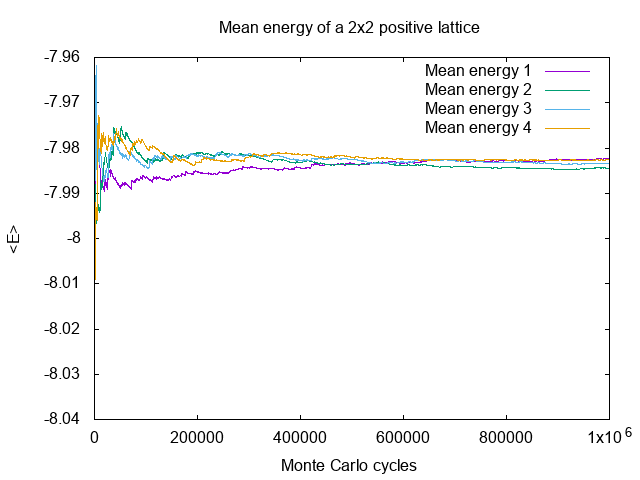
\includegraphics[width=8cm,height=6.5cm]{Results/B/T=1/Plots/energies_positive.png}
                        \end{minipage}
                        \hspace{3mm}
                        \begin{minipage}[c]{.46\linewidth}
                            \centering
                            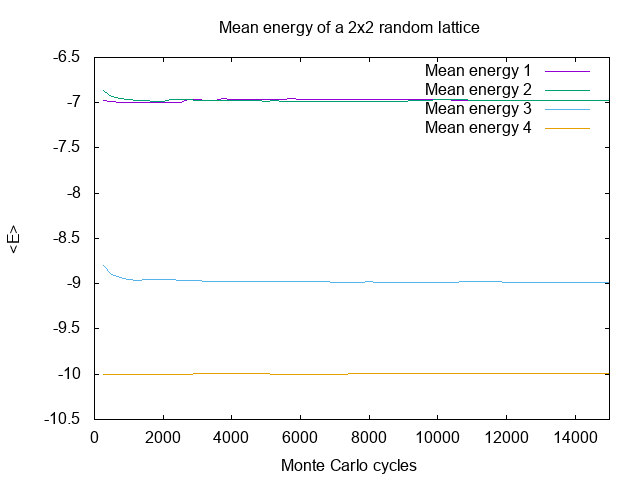
\includegraphics[width=7cm,height=6.5cm]{Results/B/T=1/Plots/energies_random.png}
                        \end{minipage}
                    }
                    \caption{The mean energy as function of the number of Monte Carlo cycles, starting with an ordered lattice (all spins-up) (left) or a random lattice (right) at $T=1$}
                \end{figure}
                \end{center}
                
            \paragraph{}The results starting with a random lattice are not exploitables as each simulation gives a different value. This is because of the size of the lattice, too small. When we begin with an ordered lattive however, the four simulations converges more or less to the same value which is nearly $-7.983$. This is totally coherent with our theorical value. \\
            For the following plots, we will only take an ordered lattice to begin.
            %
                \begin{center}
                \begin{figure}[h!]
                    \centering
                    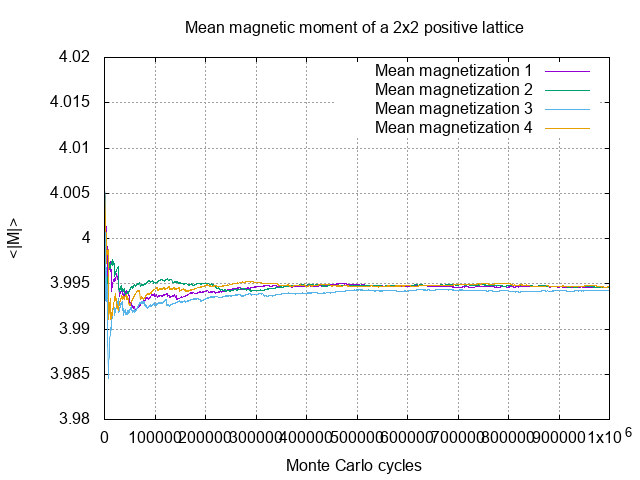
\includegraphics[width=10cm,height=6.5cm]{Results/B/T=1/Plots/Moments_positive}
                    \caption{The mean magnetic moment as function of the number of Monte Carlo cycles, starting with all spins-up over four simulations at $T=1$}
                \end{figure}
                \end{center}
            %
            We see here that this is coherent with the theorical value. The four simulations give pretty much the same value which is $\langle |M| \rangle = 3.995$ and is very close to the theorical one.
            %
                \begin{center}
                \begin{figure}[h!]
                    \centering
                    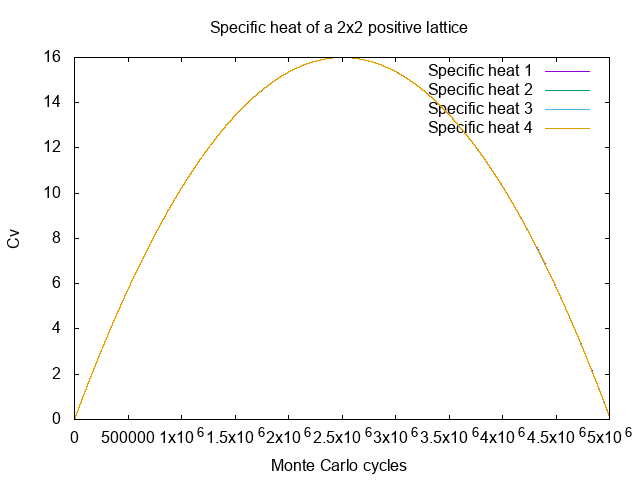
\includegraphics[width=10cm,height=6cm]{Results/B/T=1/Plots/Cv}
                    \caption{The specific heat as function of the number of Monte Carlo cycles at $T=1$}
                \end{figure}
                \end{center}
                
            \paragraph{}We have a result here which is not at all what we expected. There is no point after which the specific heat stabilizes. 
            
                \begin{center}
                \begin{figure}[h!]
                    \centering
                    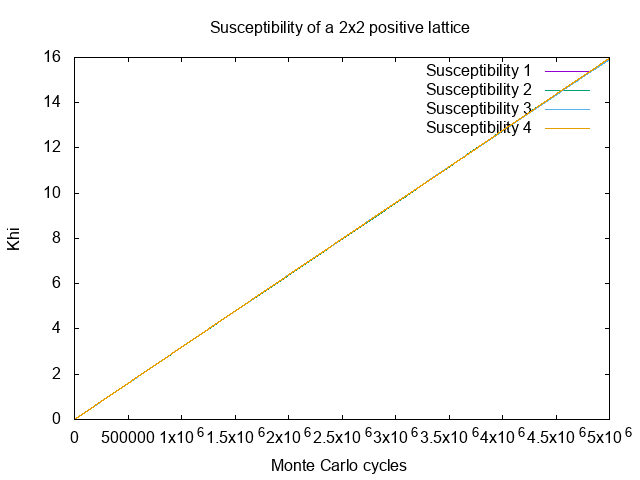
\includegraphics[width=10cm,height=8cm]{Results/B/T=1/Plots/Khi}
                    \caption{The susceptibility as function of the number of Monte Carlo cycles at $T=1$}
                \end{figure}
                \end{center}
                
            \paragraph{}Except for the mean energy and the mean magnetic moment, the results we have for the case of a $2 \times 2$ lattice at $T=1$ are obviously outliers. This may be because of the low temperature or because of the size of the lattice. We should take at least 200000 Monte Carlo cycles to reach an equilibrium situation.
            
                \begin{center}
                \begin{figure}[h!]
                    \centering
                    \hbox{
                        \begin{minipage}[c]{.46\linewidth}
                            \centering
                            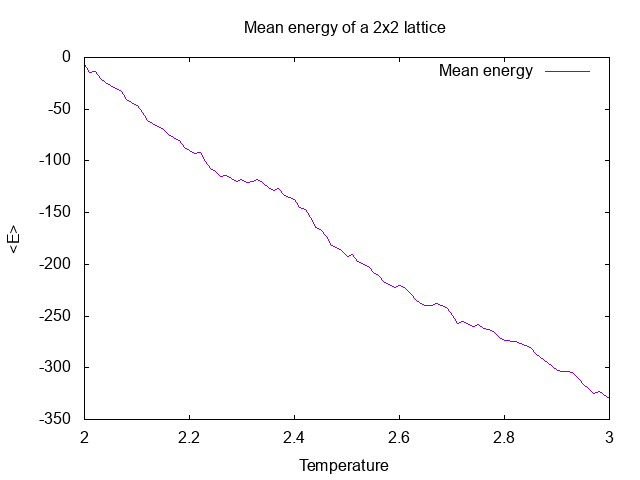
\includegraphics[width=7cm,height=5.5cm]{Results/B/Fonction_de_T/energy.png}
                        \end{minipage}
                        \hspace{3mm}
                        \begin{minipage}[c]{.46\linewidth}
                            \centering
                            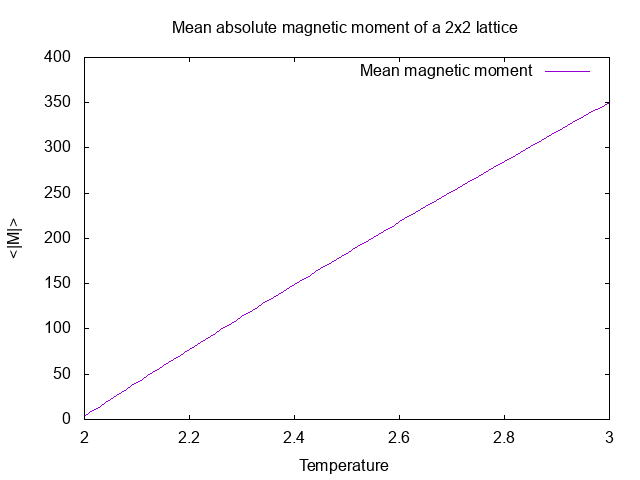
\includegraphics[width=7cm,height=5.5cm]{Results/B/Fonction_de_T/moment.png}
                        \end{minipage}
                    }
                    \caption{The mean energy and the mean magnetic moment as function of the temperature for $2 \times 10^6$ Monte Carlo cycles}
                \end{figure}
                \end{center}
                
                \begin{center}
                \begin{figure}[h!]
                    \centering
                    \hbox{
                        \begin{minipage}[c]{.46\linewidth}
                            \centering
                            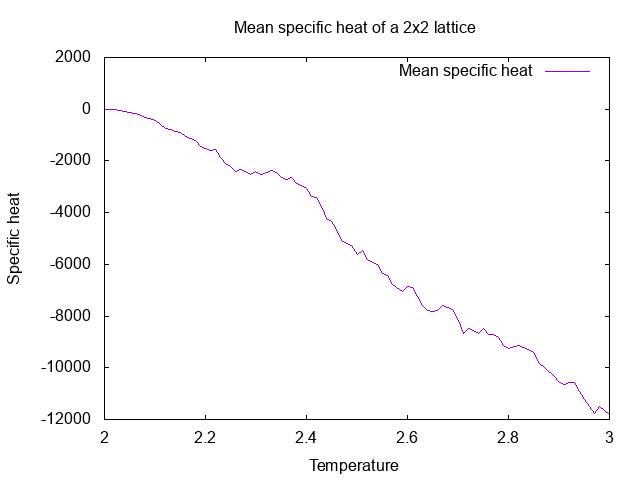
\includegraphics[width=7cm,height=5.5cm]{Results/B/Fonction_de_T/cv.png}
                        \end{minipage}
                        \hspace{3mm}
                        \begin{minipage}[c]{.46\linewidth}
                            \centering
                            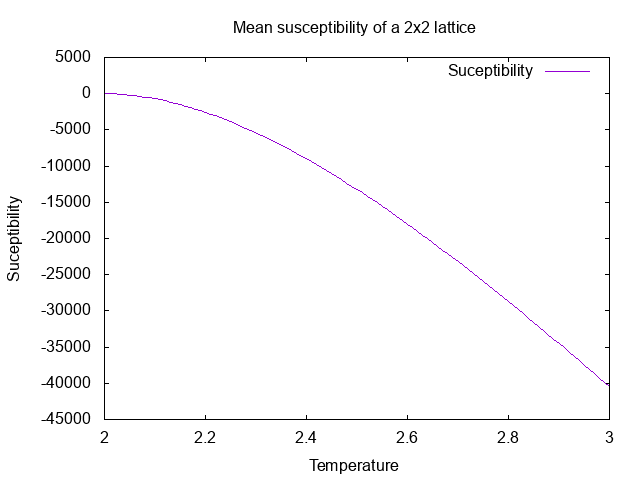
\includegraphics[width=7cm,height=5.5cm]{Results/B/Fonction_de_T/khi.png}
                        \end{minipage}
                    }
                    \caption{The specific heat and the susceptibility as function of the temperature for $2 \times 10^6$ Monte Carlo cycles}
                \end{figure}
                \end{center}
                
            \paragraph{}These results are not what I expected. The mean magnetic moment should fall at a given temperature (which is the critical temperature), the mean energy should not fall like this with the temperature.
                
            
        \subsection{$20\times20$ case}
        
            \subsubsection{Reach of the most likely state}
            
                \paragraph{}In this section we will study the time, which is here defined as the number of Monte Carlo cycles. At two different temperatures, we will run the program in order to know after how many cycles we reach an equilibrium situation. This equilibrium situation is the point at which we can begin to compute the expectation values. We will run a simulation at the temperature $T=1$ and $T=2.4$ starting with either a random lattice or an ordered one (taking all spins-up).
            
                \newpage
                \begin{center}
                \begin{figure}[h!]
                    \hbox{
                        \begin{minipage}[c]{.46\linewidth}
                            \centering
                            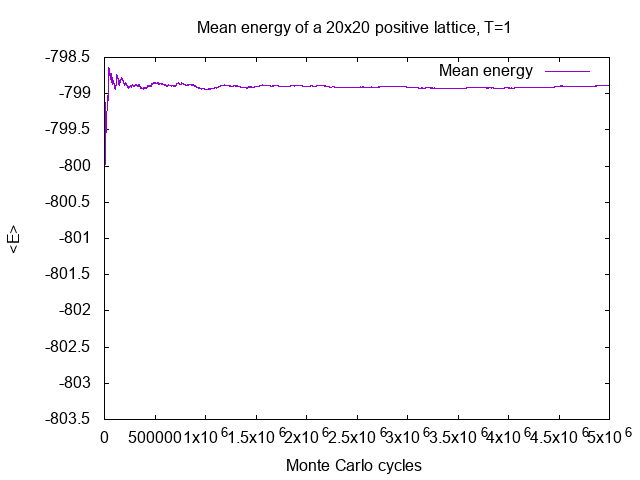
\includegraphics[width=7.5cm,height=6cm]{Results/C/T=1/Positive/energy.png}
                        \end{minipage}
                        \hfill
                        \begin{minipage}[c]{.46\linewidth}
                            \centering
                            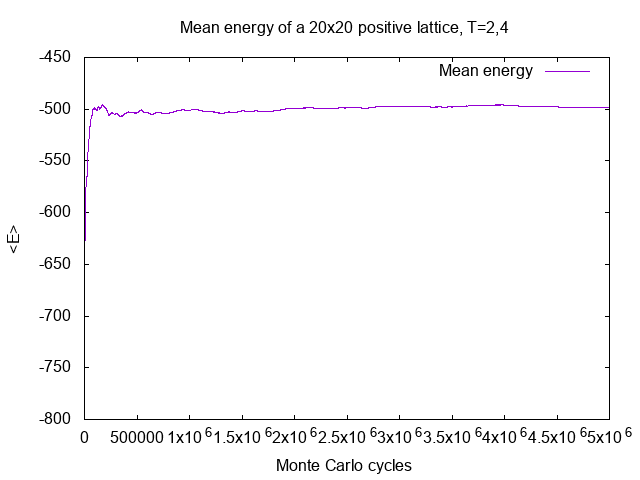
\includegraphics[width=7.5cm,height=6cm]{Results/C/T=2,4/Positive/energy.png}
                        \end{minipage}
                    }
                    \caption{The expectation value of the energy as function of the number of Monte Carlo cycles, in the case of a starting ordered lattice (all spins-up), at $T=1$ (left) and $T=2.4$ (right)}
                \end{figure}
                \end{center}
                
                
                \begin{center}
                \begin{figure}[h!]
                    \hbox{
                        \begin{minipage}[c]{.46\linewidth}
                            \centering
                            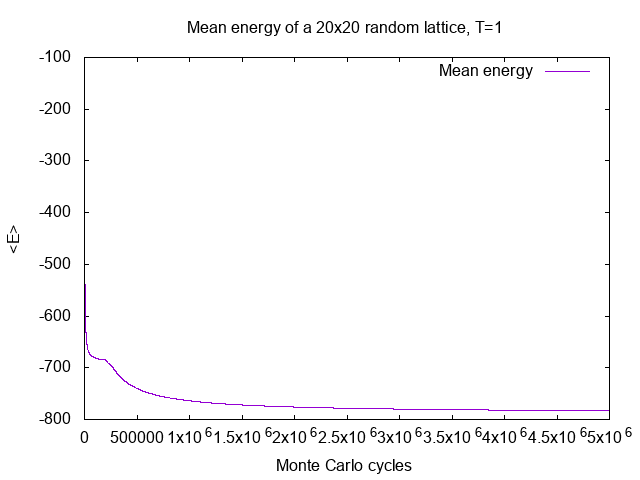
\includegraphics[width=7.5cm,height=6cm]{Results/C/T=1/Random/energy.png}
                        \end{minipage}
                        \hfill
                        \begin{minipage}[c]{.46\linewidth}
                            \centering
                            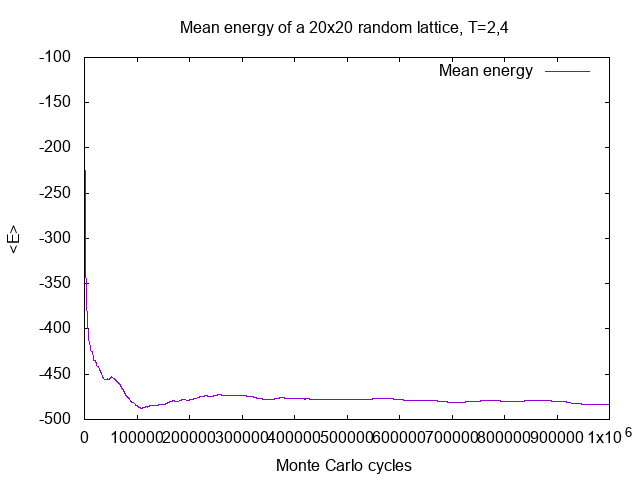
\includegraphics[width=7.5cm,height=6cm]{Results/C/T=2,4/Random/energy.png}
                        \end{minipage}
                    }
                    \caption{The expectation value of the energy as function of the number of Monte Carlo cycles, in the case of a starting random lattice, at $T=1$ (left) and $T=2.4$ (right)}
                \end{figure}
                \end{center}
                
                \paragraph{}We observe that the mean energy converges quickly to the most likely state. Approximatively, we need 500000 Monte Carlo cycles to reach an equilibrium state in the case of a low temperature ($T=1$) and pretty much the same number of cycles needed for the temperature $T=2.4$. We also observe that the mean energy is much lower for a low temperature : $\langle E \rangle_1 = 799$ against $\langle E \rangle_{2.4}=500$ which is coherent with the fact that the thermal motion increases with the temperature.\\
                Moreover, starting with an ordered lattice gives clearer results than a starting random lattice where it takes nearly $5 \times 10^6$ Monte Carlo cycles to be really stable. 
                
                \begin{center}
                \begin{figure}[h!]
                    \hbox{
                        \begin{minipage}[c]{.46\linewidth}
                            \centering
                            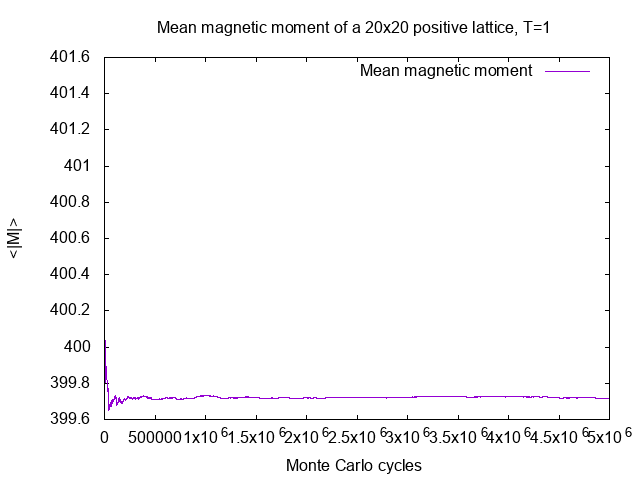
\includegraphics[width=7.5cm,height=6cm]{Results/C/T=1/Positive/moment.png}
                        \end{minipage}
                        \hfill
                        \begin{minipage}[c]{.46\linewidth}
                            \centering
                            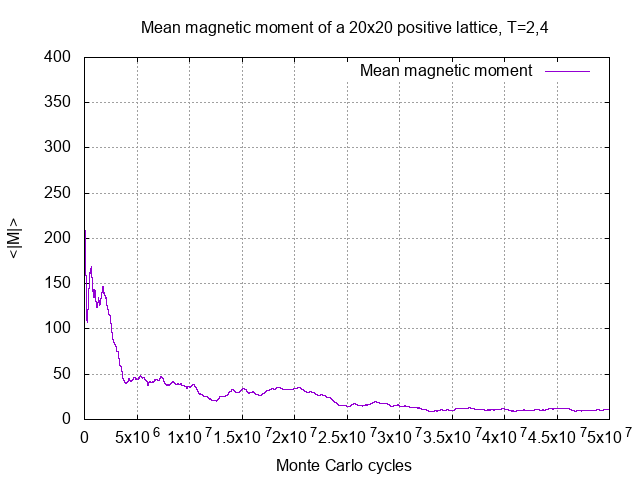
\includegraphics[width=7.5cm,height=6cm]{Results/C/T=2,4/Positive/moment.png}
                        \end{minipage}
                    }
                    \caption{The expectation value of the magnetic moment as function of the number of Monte Carlo cycles, in the case of a starting ordered lattice (all spins-up), at $T=1$ (left) and $T=2.4$ (right)}
                \end{figure}
                \end{center}
                
                
                \begin{center}
                \begin{figure}[h!]
                    \hbox{
                        \begin{minipage}[c]{.46\linewidth}
                            \centering
                            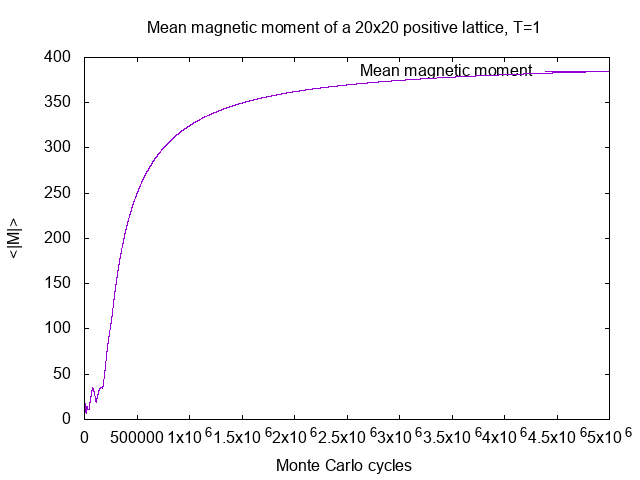
\includegraphics[width=7.5cm,height=6cm]{Results/C/T=1/Random/moment.png}
                        \end{minipage}
                        \hfill
                        \begin{minipage}[c]{.46\linewidth}
                            \centering
                            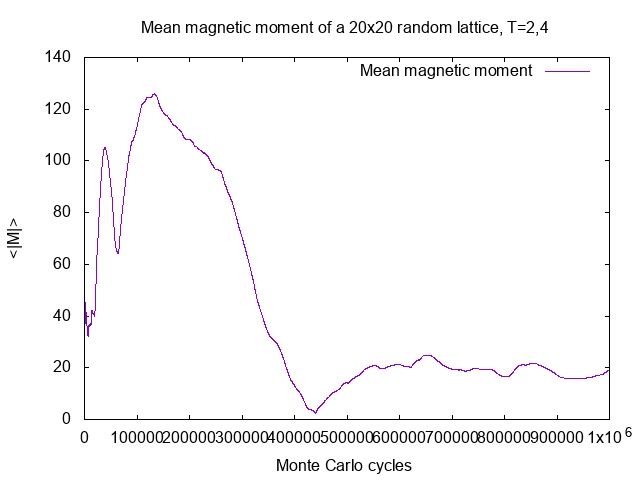
\includegraphics[width=7.5cm,height=6cm]{Results/C/T=2,4/Random/moment.png}
                        \end{minipage}
                    }
                    \caption{The expectation value of the magnetic moment as function of the number of Monte Carlo cycles, in the case of a starting random lattice, at $T=1$ (left) and $T=2.4$ (right)}
                \end{figure}
                \end{center}
            %   
            \paragraph{}The expectation value of the magnetic moment is quite stable after 250000 Monte Carlo cycles for a starting ordered lattice at $T=1$. We can compare the results with C. N. Yang's exact result published in the Physical Review 85, 808-816 in 1952, “The spontaneous magnetization of a two-dimensional Ising model”. The magnetic moment per spin is expressed as 
            
                \begin{equation*}
                    m = \left\{ \begin{matrix}
                              \left( 1-[\textnormal{sinh}(2\beta J)]^{-4} \right)^{\frac{1}{8}} & & & (T < T_C) \\
                              0 & & & (T>T_C)
                              \end{matrix}
                        \right.
                \end{equation*}
                
            So, for a $20 \times 20$ lattice, that is 400 spins, and $T=1<T_C$ we should have
            %   
                \begin{align*}
                    M_{400}&=400 \times \left(1-[\textnormal{sinh}\ 2]^{-4}\right)^{\frac{1}{8}}\\
                    M_{400}&=399.710
                \end{align*}
            %
            For $T=1$ the result we get are coherent with the value we should have. At $T=2.4$ the mean magnetization tends toward zero which means that $T=2.4>T_C$. \\
            For a random configuration as a starting configuration, the number of Monte Carlo cycles needed to be more or less stable is $1\times 10^7$. So in order to start computations of the expectation values when an equilibrium situation has been reach, we have to wait $1 \times 10^7$ Monte Carlo cycles.
            
            \paragraph{}Let's see how the number of accepted configurations evolves as function of the number of Monte Carlo cycles. 
            
                \begin{center}
                \begin{figure}[h!]
                    \hbox{
                        \begin{minipage}[c]{.46\linewidth}
                            \centering
                            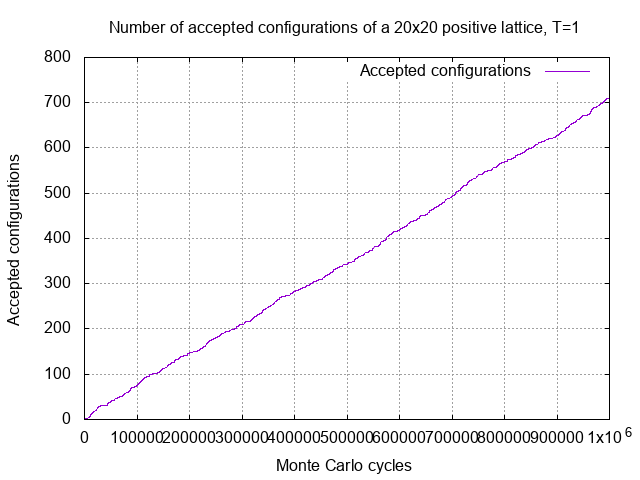
\includegraphics[width=7.5cm,height=7cm]{Results/C_et_D/T=1/Positive/configs.png}
                        \end{minipage}
                        \hfill
                        \begin{minipage}[c]{.46\linewidth}
                            \centering
                            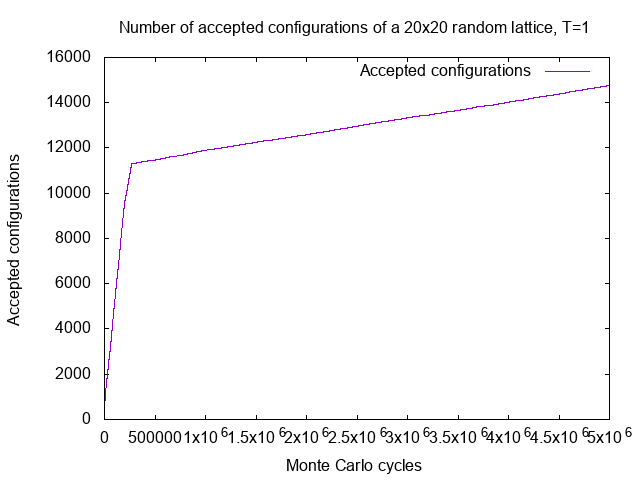
\includegraphics[width=7.5cm,height=7cm]{Results/C_et_D/T=1/Random/configs.png}
                        \end{minipage}
                    }
                    \caption{The number of accepted configurations as function of the number of Monte Carlo cycle, starting with a ordered lattice (left) or with a random one (right) at $T=1$}
                \end{figure}
                \end{center}
                
                \newpage
                \begin{center}
                \begin{figure}[h!]
                    \hbox{
                        \begin{minipage}[c]{.46\linewidth}
                            \centering
                            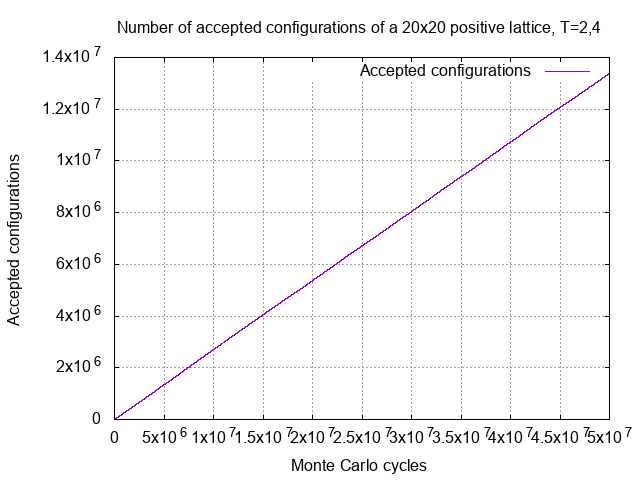
\includegraphics[width=7.5cm,height=7cm]{Results/C_et_D/T=2,4/Positive/configs.png}
                        \end{minipage}
                        \hfill
                        \begin{minipage}[c]{.46\linewidth}
                            \centering
                            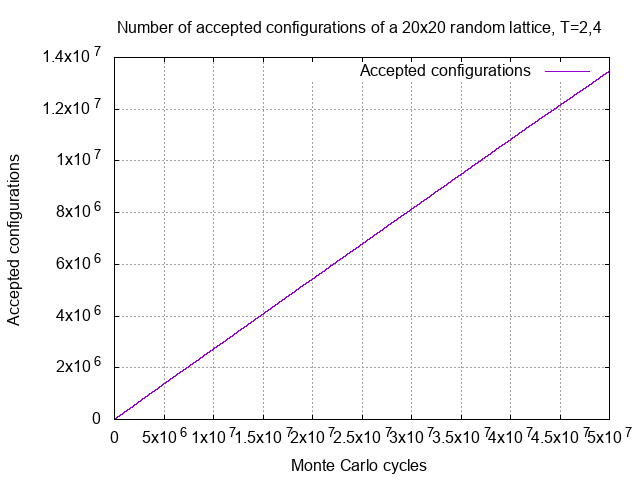
\includegraphics[width=7.5cm,height=7cm]{Results/C_et_D/T=2,4/Random/configs.png}
                        \end{minipage}
                    }
                    \caption{The number of accepted configurations as function of the number of Monte Carlo cycle, starting with a ordered lattice (left) or with a random one (right) at $T=2.4$}
                \end{figure}
                \end{center}
                
            \paragraph{}The number of accepted configurations increase lineraly with the number of Monte Carlo cycles except for a starting random configuration at the temperature $T=1$. It seems coherent as the probability of having the needed conditions to the acceptation increases with the number of Monte Carlo cycles.          
        
            \subsubsection{The probability distribution of a given energy}
            
            \paragraph{}In this section, we will looking for how many times a given energy appears in our computations. With these data, we would be able to analyze the probability distribution. 
            
                \begin{center}
                \begin{figure}[h!]
                    \hbox{
                        \begin{minipage}[c]{.46\linewidth}
                            \centering
                            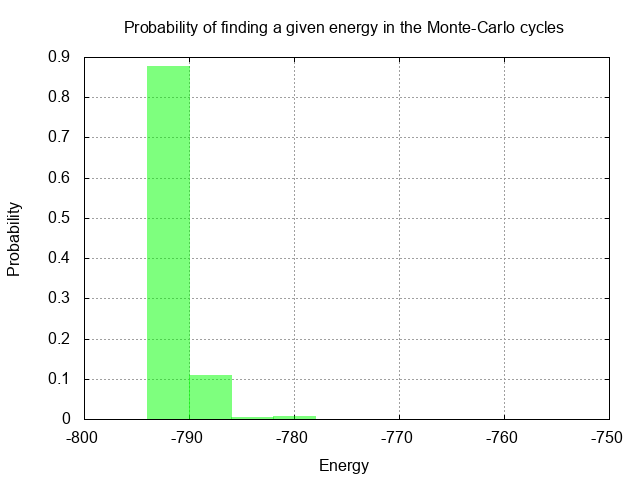
\includegraphics[width=7.5cm,height=6cm]{Results/C_et_D/T=1/Positive/energies_proba.png}
                        \end{minipage}
                        \hfill
                        \begin{minipage}[c]{.46\linewidth}
                            \centering
                            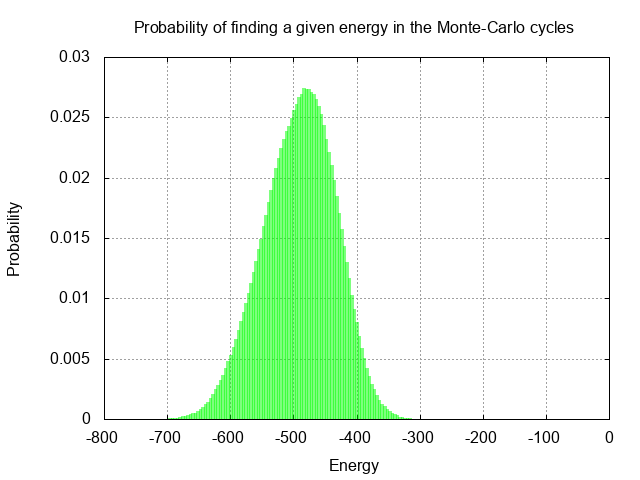
\includegraphics[width=7.5cm,height=6cm]{Results/C_et_D/T=2,4/Positive/energies_proba.png}
                        \end{minipage}
                    }
                    \caption{The probability distribution $P(E)$}
                \end{figure} 
                \end{center}          
            
            \paragraph{}At low temperature, we have very few possible values for the energy, the curve is centered near the expectation value of the energy. At temperature $T=2.4$, the Gaussian distribution is way more extended. We have more possible values. The curve is centered at the expectation value we have determined above. \\
            The variance in energy for $T=1$ are really big whereas we expected low variances because the curve is not extended. The variance at $T=2.4$ are smaller but still very big.
            
\newpage
    \section{Phase transitions}
    
        \subsection{The Ising model near the critical temperature}
        
            \paragraph{}We will focus on a smaller interval around a supposed critical temperature : $T \in [2.0,2.3]$. We take different size for the lattice : $L=40$, $L=60$, $L=80$ and $L=100$.
            
                \begin{center}
                \begin{figure}[h!]
                    \hbox{
                        \begin{minipage}[c]{.46\linewidth}
                            \centering
                            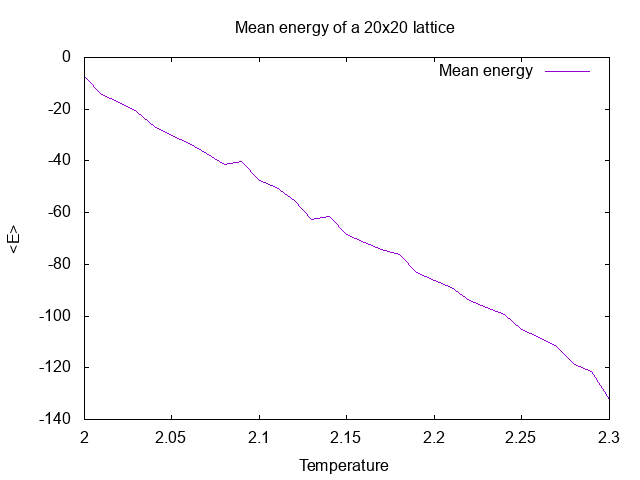
\includegraphics[width=7.5cm,height=7cm]{Results/E/L=40/energy.png}
                        \end{minipage}
                        \hfill
                        \begin{minipage}[c]{.46\linewidth}
                            \centering
                            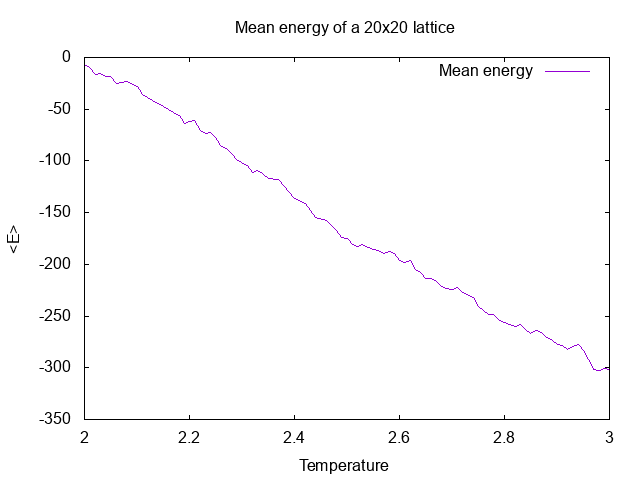
\includegraphics[width=7.5cm,height=7cm]{Results/E/L=60/energy.png}
                        \end{minipage}
                    }
                \end{figure} 
                \end{center}
                
                \begin{center}
                \begin{figure}[h!]
                    \hbox{
                        \begin{minipage}[c]{.46\linewidth}
                            \centering
                            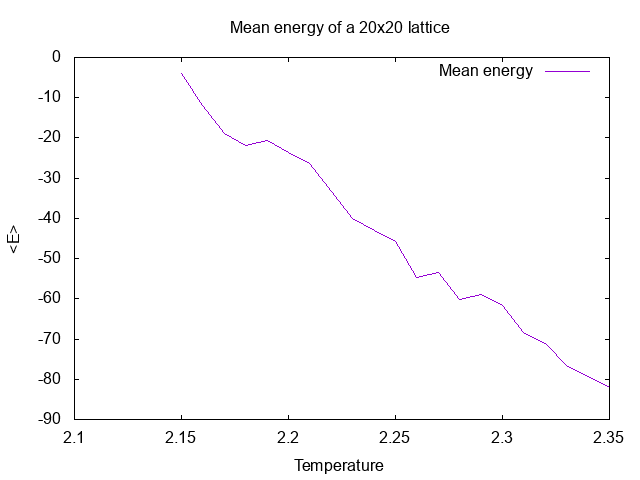
\includegraphics[width=7.5cm,height=6cm]{Results/E/L=80/energy.png}
                        \end{minipage}
                        \hfill
                        \begin{minipage}[c]{.46\linewidth}
                            \centering
                            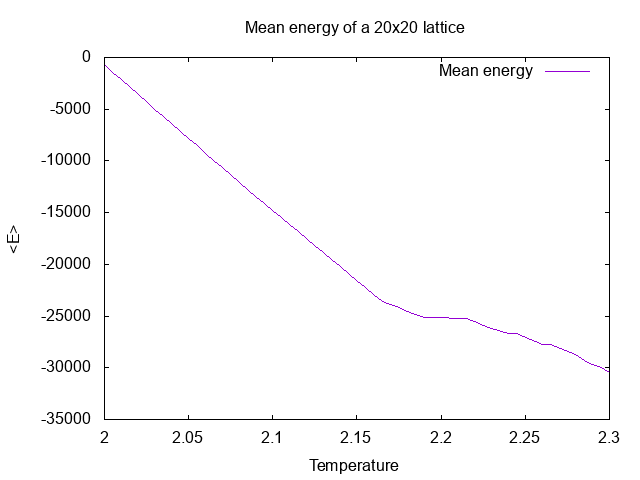
\includegraphics[width=7.5cm,height=6cm]{Results/E/L=100/energy.png}
                        \end{minipage}
                    }
                    \caption{The mean energy as function of the temperature near the critical temperature for $L=40, 60, 80, 100$}
                \end{figure} 
                \end{center}
                
                \begin{center}
                \begin{figure}[h!]
                    \hbox{
                        \begin{minipage}[c]{.46\linewidth}
                            \centering
                            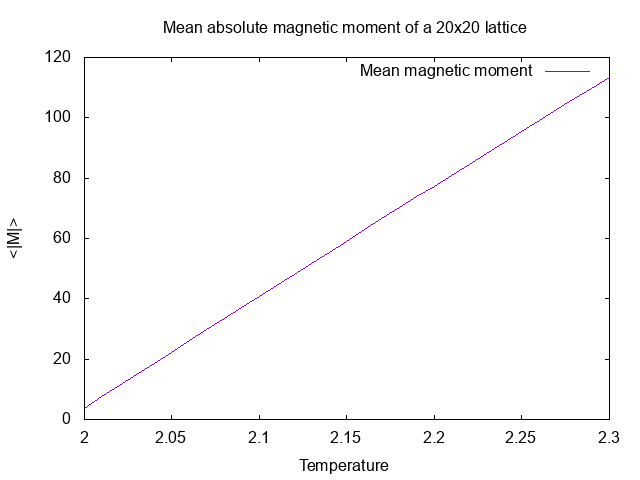
\includegraphics[width=7.5cm,height=6cm]{Results/E/L=40/moment.png}
                        \end{minipage}
                        \hfill
                        \begin{minipage}[c]{.46\linewidth}
                            \centering
                            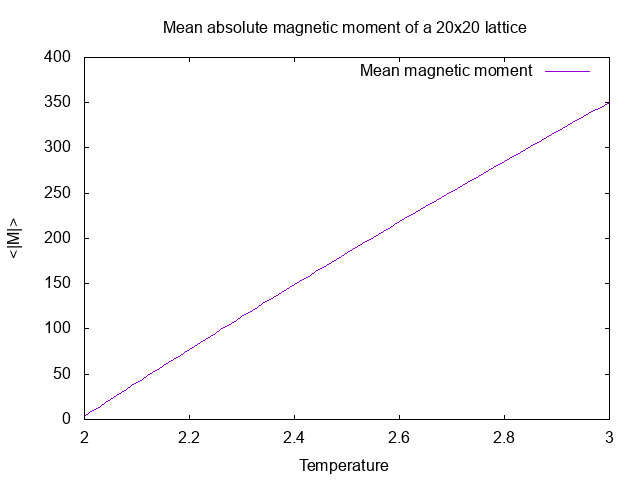
\includegraphics[width=7.5cm,height=6cm]{Results/E/L=60/moment.png}
                        \end{minipage}
                    }
                \end{figure} 
                \end{center}
                
                \begin{center}
                \begin{figure}[h!]
                    \hbox{
                        \begin{minipage}[c]{.46\linewidth}
                            \centering
                            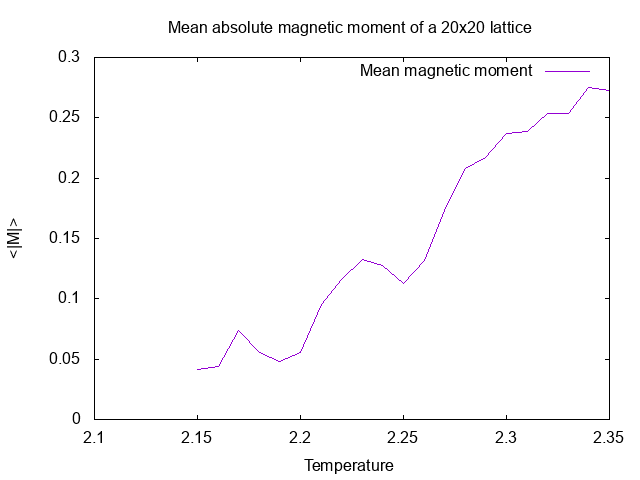
\includegraphics[width=7.5cm,height=6cm]{Results/E/L=80/moment.png}
                        \end{minipage}
                        \hfill
                        \begin{minipage}[c]{.46\linewidth}
                            \centering
                            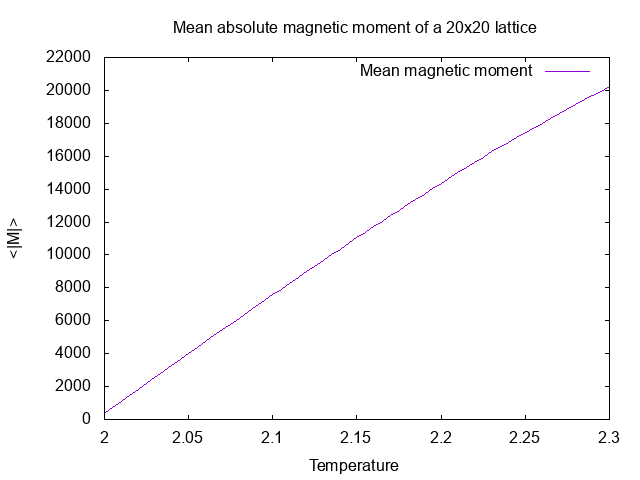
\includegraphics[width=7.5cm,height=6cm]{Results/E/L=100/moment.png}
                        \end{minipage}
                    }
                    \caption{The mean magnetic moment as function of the temperature near the critical temperature for $L=40, 60, 80, 100$}
                \end{figure} 
                \end{center}
                
                \begin{center}
                \begin{figure}[h!]
                    \hbox{
                        \begin{minipage}[c]{.46\linewidth}
                            \centering
                            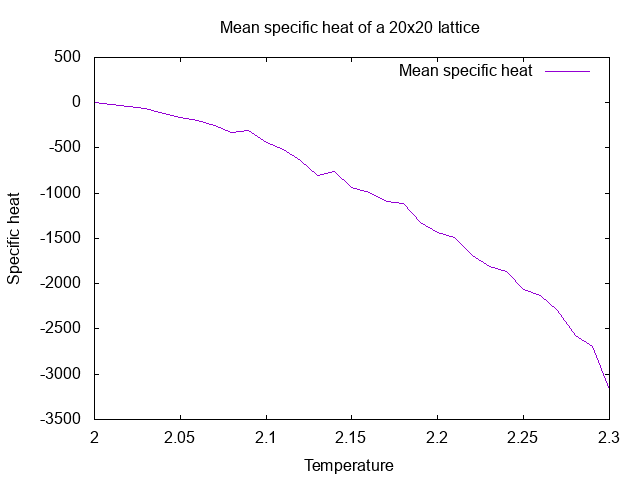
\includegraphics[width=7.5cm,height=6cm]{Results/E/L=40/cv.png}
                        \end{minipage}
                        \hfill
                        \begin{minipage}[c]{.46\linewidth}
                            \centering
                            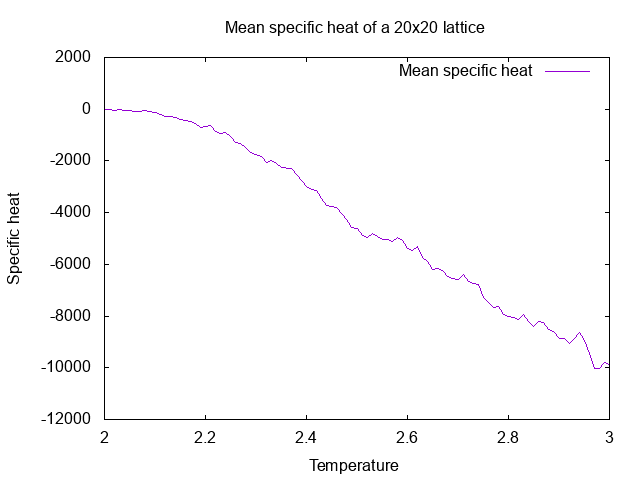
\includegraphics[width=7.5cm,height=6cm]{Results/E/L=60/cv.png}
                        \end{minipage}
                    }
                \end{figure} 
                \end{center}
                
                \begin{center}
                \begin{figure}[h!]
                    \hbox{
                        \begin{minipage}[c]{.46\linewidth}
                            \centering
                            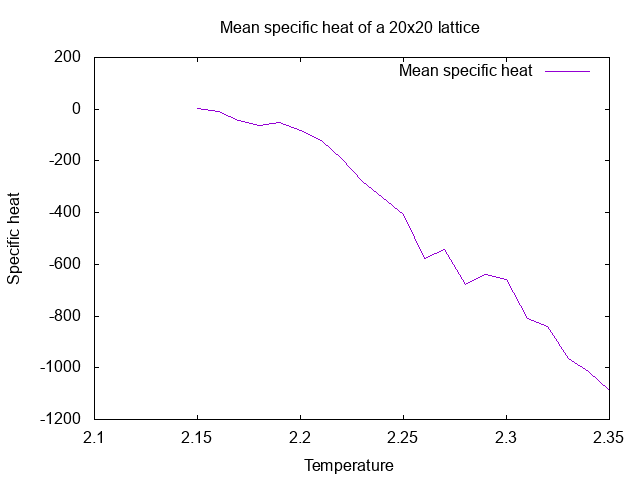
\includegraphics[width=7.5cm,height=6cm]{Results/E/L=80/cv.png}
                        \end{minipage}
                        \hfill
                        \begin{minipage}[c]{.46\linewidth}
                            \centering
                            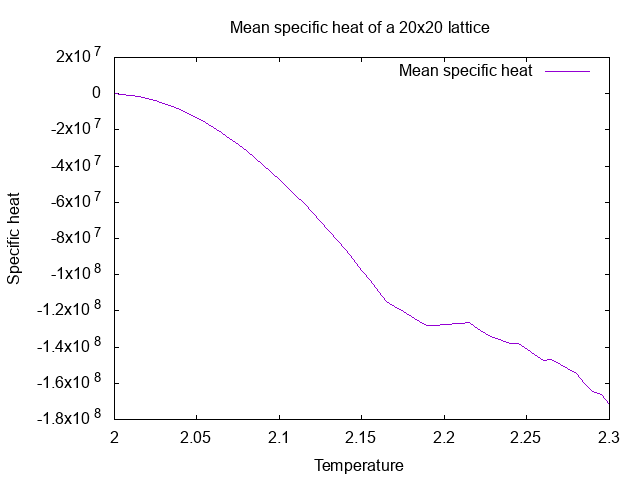
\includegraphics[width=7.5cm,height=6cm]{Results/E/L=100/cv.png}
                        \end{minipage}
                    }
                    \caption{The specific heat as function of the temperature near the critical temperature for $L=40, 60, 80, 100$}
                \end{figure} 
                \end{center}
                
                \begin{center}
                \begin{figure}[h!]
                    \hbox{
                        \begin{minipage}[c]{.46\linewidth}
                            \centering
                            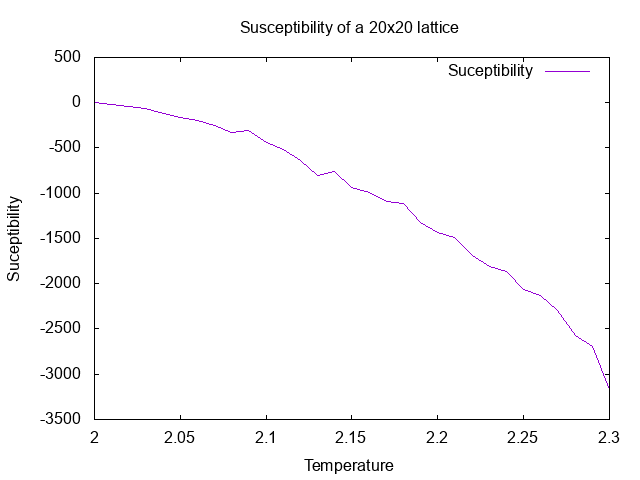
\includegraphics[width=7.5cm,height=6cm]{Results/E/L=40/khi.png}
                        \end{minipage}
                        \hfill
                        \begin{minipage}[c]{.46\linewidth}
                            \centering
                            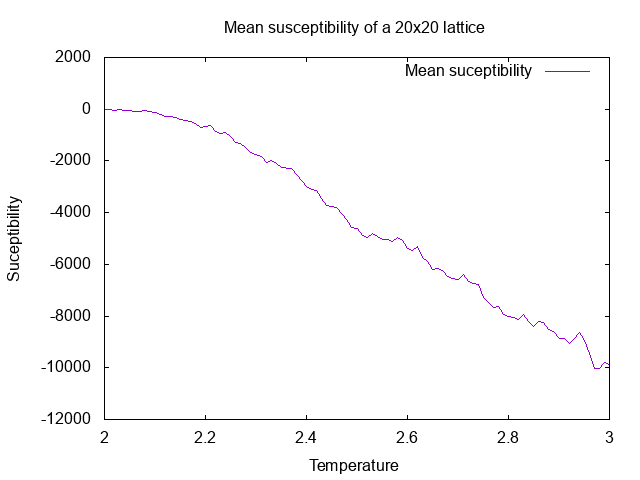
\includegraphics[width=7.5cm,height=6cm]{Results/E/L=60/khi.png}
                        \end{minipage}
                    }
                \end{figure} 
                \end{center}
                
                \begin{center}
                \begin{figure}[h!]
                    \hbox{
                        \begin{minipage}[c]{.46\linewidth}
                            \centering
                            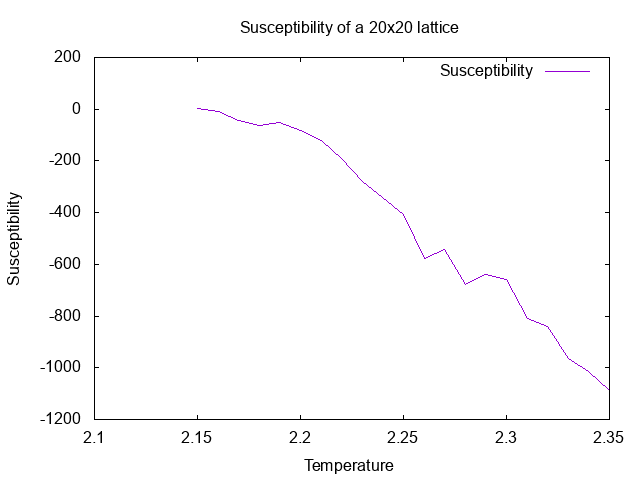
\includegraphics[width=7.5cm,height=6cm]{Results/E/L=80/khi.png}
                        \end{minipage}
                        \hfill
                        \begin{minipage}[c]{.46\linewidth}
                            \centering
                            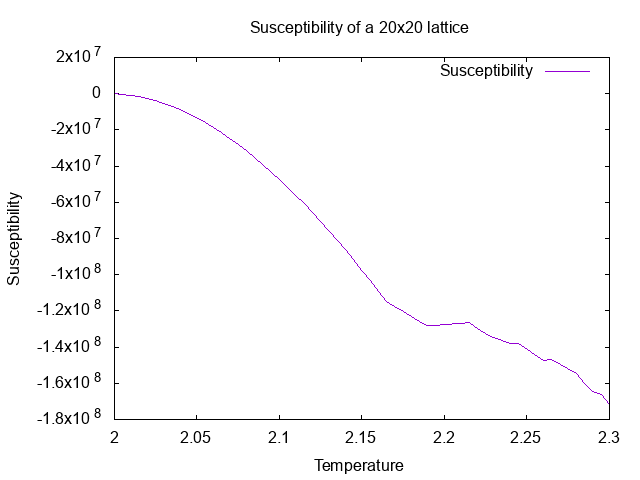
\includegraphics[width=7.5cm,height=6cm]{Results/E/L=100/khi.png}
                        \end{minipage}
                    }
                    \caption{The susceptibility as function of the temperature near the critical temperature for $L=40, 60, 80, 100$}
                \end{figure} 
                \end{center}
                
            \paragraph{}We, again, do not have what we expected. We should see the phase transition on these plots. For example, the susceptibility should diverge at $T_C$. We are not able to find the critical temperature with these simulations.
            
        \newpage
        \subsection{The critical temperature}



\chapter*{Conclusion}
\addcontentsline{toc}{chapter}{Conclusion}

    \paragraph{}
    

\chapter*{Bibliography}
    
    \begin{itemize}
        \item Lars Onsager Phys. Rev. 65, 117 (1944)
        \item C. N. Yang, “The spontaneous magnetization of a two-dimensi
onal Ising model,” Phys.  Rev.85, 808–816 (1952)
    \end{itemize}
    

\end{document}